%%%astrophysics stuff like redshift??
Some astrophysics terms and constants:

\begin{itemize}
    \item z - redshift
    \item H - the Hubble constant
    \item h
    \item G - gravitational constant

\end{itemize}

\subsection{Galaxy formation}

Our understanding of the formation and evolution of the universe as a whole is based on the cosmological principle, which states that matter is distributed spatially isotropically and homogeneously across the universe on large scales. Of course, we would not have any structure formation if the matter was actually perfectly uniformly distributed in the very beginning of the universe. It is not completely clear how this initial deviation from homogenity originated, but at very early times after the Big Bang, the universe was so small that quantum effects would have played a significant role. These tiny quantum fluctuations may then have been responsible for the initial structure formation we can observe today.

Given that these initial density fluctuations in matter were present, gravitational effects will then amplify the overdense regions of space as matter is pulled together. If the universe did not expand, these instabilities in the density field would just keep growing. However, we know the universe is expanding, and so the effect is dampened significantly. At a point in time, the overdense region will reach a ``turn-around size'' where the gravitational potential is large enough to over compensate for the expansion rate of space. Then the matter will collapse towards the center. The excact process for collapse is beyond the scope of this report, but it depends on the ratio of dark matter to baryonic matter, and the properties of the dark matter itself. 

\subsubsection{Dark matter halos}
Dark matter halos are the result of such initial overdense regions of dark matter particles. Halos cover a huge range in magnitudes of mass from $M_{halo} <10^9 M_{\odot}$ to $M_{halo} >10^{15} M_{\odot}$. In general, halos are ellipsoid in shape. The spherically averaged density profile of halos, as predicted by N-body simulations of dark matter in a $\Lambda$CDM universe, is well described by the Frank-Nevarro-White profile \parencite{Navarro1996},
\begin{equation}
    \frac{\rho}{\rho_{crit}} = \frac{\delta_c}{(r/r_c)(+1+r/r_s)^2.}
\end{equation}
$\rho_{crit} = 3H^2/8\pi G$ is the critical density, $\delta_c$ is the characteristic overdensity and $r_s$ is the scale radius. Both $\delta_c$ and $r_s$ may vary for each halo.

Halos grow hierarchically through mergers of smaller halos into larger halos. A smaller halo that merges with a larger halo may survive as a seperate entity within the host halo and is then known as a subhalo. 

One of the most interesting properties of a $\Lambda$CDM universe is the halo mass function, the number density of halos as a function of their mass. In a famous paper by William H. Press and Paul Schechter \parencite{Press1974}, the halo mass function is defined as:

\begin{equation}
    \frac{dn}{dM} = f(\sigma)\frac{\overline{\rho}}{M^2}\frac{d\log(\sigma^{-1})}{d\log(M)}.
\end{equation}

Where $f(\sigma)$ is the multiplicity function, $\sigma (R)$ is the variance of the field with a smoothing radius R, and $\overline{\rho}$ is the mean density of the universe. In that paper, the multiplicity function was given as

\begin{equation}
    f(\sigma) = \frac{2}{\pi} \sigma \exp(-\sigma^2/2).
\end{equation}

We will not cover the mathematical details of this analytical solution to the mass function, but it is based on the assumption of spherical collapse, and is not dependent on cosmology or redshift. Until the end of the century, numerical simulations tended to agree with the 1974 results. However, newer and more complex numerical solutions have shown that the Press-Schechter formalism tends to overestimate the amount of smaller halos, while underpredicting the abundance of larger halos. There has also been several studies that show how the mass function actually is slightly redshift-dependent (e.g. \cite{Tinker2008}).

\subsubsection{Galaxies}
As dark matter halos formed in the very early universe, they created a graviational potential well which gave room for the primordial baryonic matter (ionized hydrogen gas) to start collapsing. As the density of the gas increased, temperature increased and halted the collapse, but through several radiation cooling processes the gas was able to collapse enough for fusion to start and stars to be born. Because of the halos role as initial potential wells, the baryonic matter collapsed in such a way that it formed a spinning disk around the center of the halo. This was the birth of galaxies as we know them today.

Galaxies are mainly composed of stars and hot gas, with a smaller contribution of stellar remnants, cold gas and dust. Hot gas is hydrogen gas that is fully ionized, and does not collapse into stars, while cold gas has a much lower temperature and can contribute to star formation. There are at least two trillion galaxies in the observable universe \parencite{Conselice2016}, with stellar masses ranging from $<10^6 M_{\odot}$ to $10^\{12\} M_{\odot}$. 

It has been found that a large fraction of the galaxies are gravitationally bound to each other in groups and clusters. % (Geller& Huchra 1989; Bond et al. 1996) 
Galaxy clusters are the largest gravitationally bound systems in the Universe, and can span a distance of several megaparsecs. They typically contain more than a hundred galaxies, as well as large amounts of intergalactic gas. Galaxies in galaxy clusters serve an important purpose to astrophysicists, as they essentially function as tracors of the largest halos in the universe.

The $\Lambda$CDM model for our universe gives a bottom-up solution to galaxy formation, a hierarchical formation. Essentially this means that larger galaxies have formed through mergers of smaller galaxies. When a galaxy forms, the angular momentum of its initial components get transferred to the galaxy as a whole, and the result is a rotating disk galaxy. Galaxies that are not pure disk galaxies, but have an elliptical component og stars and gas with a pressure dominated random motion and which extends in all directions from the center, are results of the merging of galaxies. As many galaxies exist in clusters, the likelihood of a galaxy merger is higher than one might otherwise expect in those regions, and so galaxy clusters contain more elliptical galaxies.

A very important property of the galaxy population is the galaxy luminosity function, which gives the number density of galaxies as a function of their luminosity. The luminosity of a galaxy is directly proportional to its stellar mass, so the luminosity function also gives us the mass distribution of galaxies. Mathematically, the luminosity function is defined as $\phi(L)dL$, the number density of galaxies in the luminosty range $L \pm dL/2$. In 1976 Paul Schechter proposed a fit to the luminosity function of galaxies on the form

\begin{equation}
    \phi(L)dL = \phi^*(L/L^*)^{\alpha}\exp{(-L/L^*)}dL/L^*,
\end{equation}

where $\phi^*$ is a normalization, $L^*$ is the characteristic luminosity for that sample of galaxies (it will differ for instance for galaxies within a c luster compared to isolated galaxies) and $\alpha$ is the slope of the power law where $L<<L^*$ \parencite{Schechter1976}. This Schechter function is still a good fit to this day, and is in excellent agreement for galaxies with $L>>L^*$. For the low mass range of galaxies, the parameter $\alpha$ must be found, and this is one of the challenges of astrophysicists that study galaxy properties.


\subsubsection{Stellar-to-Halo mass relation}
%The technique consist in assuming that the most massive galaxy lives in the most massive halo, that the second most massive galaxy lives in the second most massive %halo, and so on. in practice, this is done by matching the abundances between the "halo mass function" and the "luminosity function of galaxies".
%The "luminosity function" can be measured observationally, because we can see galaxies. But "halo mass function" come from simulations, because we can not observe Halos.

The stellar-to-halo mass relation (SHMR) is a relation which gives the stellar mass of a galaxy as a function of its host halo mass. This is particularly difficult to find empirically, as it is not possible to directly measure the dark matter halo mass. 

One way of looking for this relation is through a method called abundance matching. In abundance matching, the numerically found halo mass function and the observationally found luminosity function are combined. This is done using the simple assumption that the largest halo contains the largest galaxy, the second largest halo contains the second largest halo and so on. By mapping each galaxy to its corresponding halo in such a fashion, the shape of the SHMR can be found directly.

Using abundance matching, the SHMR has been found to be well described by a power law for low-mass galaxies, and a subpower law for the high-mass end of the spectrum \parencite{Behroozi2013}. 

\begin{equation}
    \log(M_*(M_h)) = \log(\epsilon M_1) + f(\log(M_h/M_1)) -f(0),
\end{equation}
\begin{equation*}
    f(x) = -\log(10^{\alpha x}+1)+\delta \frac{(\log(1+\exp(x)))^\gamma}{1 +\exp(10^{-x})}
\end{equation*}

Here $M_*$ is the stellar mass, $M_h$ is the halo mass, $M_1$ is a characteristic halo mass, $\delta$ is the strength of the subpower law, $\alpha$ is the power law slope for $M_h << M_1$ and $\gamma$ is the power law index for $M_h >> M_1$.

Other ways of studying the SHMR is through simulations which include both the halo mass and the corresponding stellar mass for that halo, or through inferring the halo mass by using the rotational curves of disk galaxies (see section \ref{earlies}).

\subsection{Galaxy evolution and classification}
%Maybe make list/figure to sum up differences
As soon as telescopes became good enough to clearly make out galaxies in the sky, it became apparent to astronomers that galaxies come in many different shapes and sizes. The morphology of a galaxy is important because it turns out that morphology is closely linked to other properties of the galaxy. Edwin Hubble classified galaxies on a spectra \parencite{Hubble1926}, with elliptical galaxies (galaxies that have a dominant spheroidal component) on one end of the spectrum and spiral galaxies (galaxies with a prominent disk component) on the other (see Figure \ref{hubble}). As the galaxy types were presented as a sequence, Hubble deemed it convenient to use the adjectives ``early'' and ``late'' to describe the two extreme ends of the spectrum. He did consider the fact that these words might be confusing because of their temporal connotations, but went ahead with using ``early'' and ``late'' as a proxy for ``less complex'' and ``more complex'', respectively. Indeed this turned out to be confusing, as it is now established that galaxies actually evolve with time along the sequence, starting out as late-type disk galaxies and often ending up as more massive early-type ellipticals.

\begin{figure}
    \centering
    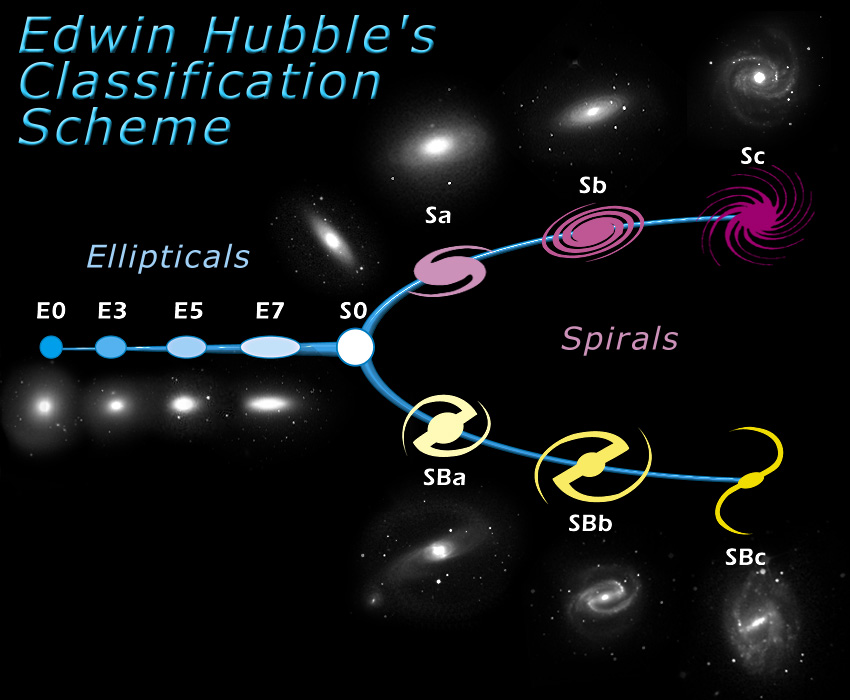
\includegraphics[width=0.9\textwidth]{images/hubble.jpg}
    \caption{Chart from 1999 showing the original classifications of galaxy morphology. Credit: ESA/Hubble}
    \label{hubble}
\end{figure}

In the $\Lambda$CDM model, galaxies grow through mergers. Mergers are separated into two types, major and minor mergers.  Major mergers are events where two galaxies of equal size collide and become one galaxy. Simulations have shown that a major merger between two disk galaxies produces an elliptical. The Milky Way, which is a large spiral galaxy ($M_*>10^{10}$) has probably grown through many smaller minor mergers, and thus kept its disky part.

It is not always easy to distinguish between a disky elliptical and a spiral with a large spheroidal component (bulge). Some galaxies are also in the middle of a merging process. These can have very irregular shapes, and so are hard to classify. Other galaxies are very small, so called dwarf galaxies. These galaxies tend to have very little stellar mass compared to dark matter, so they do not exhibit the properties of ellipticals, even though they may be more elliptical in shape.

\subsubsection{Elliptical (early type) galaxies}
Elliptical galaxies are mainly pressure-dominated systems, meaning that the motion of the stars is predominantly radial. The largest galaxies in the universe tend to be ellipticals, but they come in all sizes. The star population of ellipticals is generally older than that of spirals, and there is usually little to no star formation. There is very little gas and dust in ellipticals, and they tend to emit more light in the redder end of the EM spectrum. Early type galaxies are less common than late type galaxies, and are more usually found in galaxy clusters.

\subsubsection{Spiral (late type) galaxies} \label{earlies}
Late type galaxies have a prominent disky component, orbiting around the galaxy's center. The rotational velocity of the disk is typically much larger than the velocity dispersion of the galaxy's bulge. The stars in a spiral galaxy are usually much younger than those in early types. There is a lot of gas and dust present in spirals, giving rise to ongoing star formation. Late type galaxies are bluer in color than early types. Field galaxies, galaxies that are not part of a galaxy cluster, are predominantly spirals. 


The rotational velocities of the stars at different radii in the disk of spiral galaxies can be measured observationally, and plotting the velocity as a function of radius gived us the velocity curve og the galaxy. If the mass in the galaxy was solely made up of the gas and stars that we are able to detect optically, we would expect the velocity curve to drop off as we get to the outer parts of the galaxy. Assuming the particles move in circular orbits around the center of mass, the circular velocity at a given radius is given by the formula

\begin{equation}
    v_{circ} = \sqrt{GM(<R)/R}. 
\end{equation}

However, the observational data shows that the velocity curve does not fall off towards the outer parts of the galaxy, but actually flattens out (see Figure \ref{rotation_curves}). This perplexed early astrophysicists, as the mass inside the outer radii must be much greater than that which could be accounted for by the stars and gas in the galaxy. An effort to solve this problem led to the theory of dark matter, and later to the $\Lambda$CDM model.

\begin{figure}
    \centering
    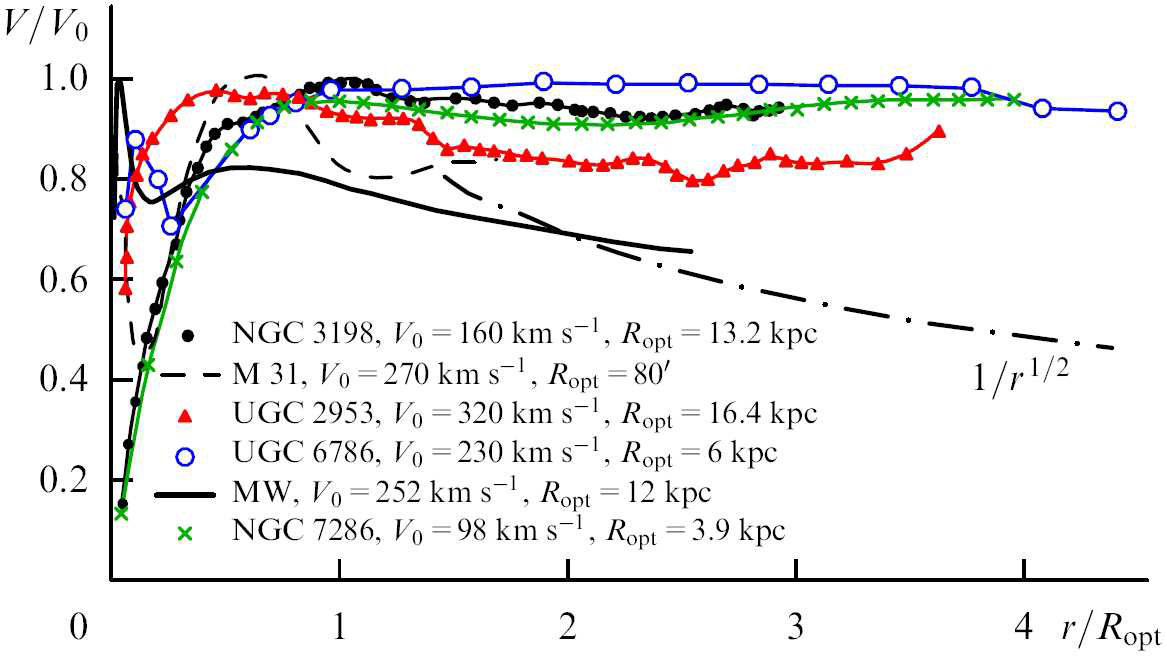
\includegraphics[width=0.9\textwidth]{images/rotation_curves.png}
    \caption{Rotation curves for several spiral galaxies. The dashed line is the expected curve if there was no dark matter. Credit: \cite{Zasov2017}}.
    \label{rotation_curves}
\end{figure}

The main differences between early and late-type galaxies is summed up in table \ref{morphologies}.

\begin{table}
\begin{center}
\begin{tabular} { l| c c } 
 \hline
 \hline
  & Early type & Late type \\
 \hline
 Shape & Spheroidal & Disk \\
 Color & Red & Blue \\
 Velocity direction& radial & circular \\
 Stellar population & older & younger \\
 Star formation rate & low & high \\
 Size & smaller & larger \\
 Gas and dust & little & much \\
  
 \hline 
\end{tabular}
\end{center}
\caption{Galaxy properties by morphology type}
\label{morphologies}
\end{table}

\subsection{Galaxy properties}
%Are you going to show a plot in each of the following  sub-sections ? 
%You should also say that all this correlations are studied in all possible redshift range (not only z=0)


\subsubsection{The Tully-Fisher relation}

In 1977, R.B. Tully and J.R. Fisher \parencite{TullyFisher1977} published a paper where they found a surprisingly good correlation between the luminosity of a spiral galaxy and the characteristic rotational speed of its disk on the form of a simple power law with index $\alpha$.

\begin{equation}
    L \propto v_{rot}^\alpha
\end{equation}
%alpha = 4 
This is known as the Tully-Fisher relation (TFR). As stellar mass is directly proportional to the luminosity, this gives us the ability to estimate stellar mass from a simple measurement of the rotational velocity.

\begin{equation}
    M_* \propto v_{rot}^\alpha 
\end{equation}

The power law index $\alpha$ was found to be 3.7. Later work has found $\alpha$ to lie between 3.5 and 4 (needs citing...).

This relation is a great tool for estimating the distance to a galaxy, as the calculated luminosity can be compared to the observed luminosity at Earth. For numerical simulations, being able to reproduce the TFR is an essential way to check if the model used is reliable.

\subsubsection{The Faber-Jackson relation and the Fundamental Plane}
At around the same time that Tully and Fisher published their paper, Sandra M. Faber and Robert Earl Jackson published a paper that linked the velocity dispersion and luminosity of early-type galaxies. The proposed relation was on the form of a power law as well,

\begin{equation}
    L \propto \sigma^{\gamma},
\end{equation}

with a power law index $\gamma$ of approximately 4 \parencite{FaberJackson1976}.

This is known as the Faber-Jackson (FJ) relation. The scatter in the FJ relation was larger than that found for the TFR however, and it was later found that the velocity dispersion also was dependent on the size of the galaxy.

\begin{equation}
    \sigma \propto L^a R^b
\end{equation}

With the radius added into the equation, the scatter became much less significant. Most ellipticals are found on the same plane in ${\sigma, R, L}$ space. This plane became known as the Fundamental Plane (FP), through a paper published in 1987 \parencite{Djorgovski1987}, and is also something which successfull numerical simulations must reproduce.

\subsubsection{Color bimodality}
Color, in astrophysics, is defined as the difference in magnitudes measured for a galaxy by two different optical filters. A galaxy that is "blue" has a larger amount of blue light than red. In general, galaxies are found to inhabit one of two groups on a color-mass diagram, blue and red (see Figure \ref{color_bimodality}). The blue galaxies are most often smaller late type galaxies, while the red ones are mainly larger early types. There are many factors that contribute to the color of a galaxy, like stellar age and metallicity as well as the amount of gas the light has passed through and its metallicity.

\begin{figure}
    \centering
    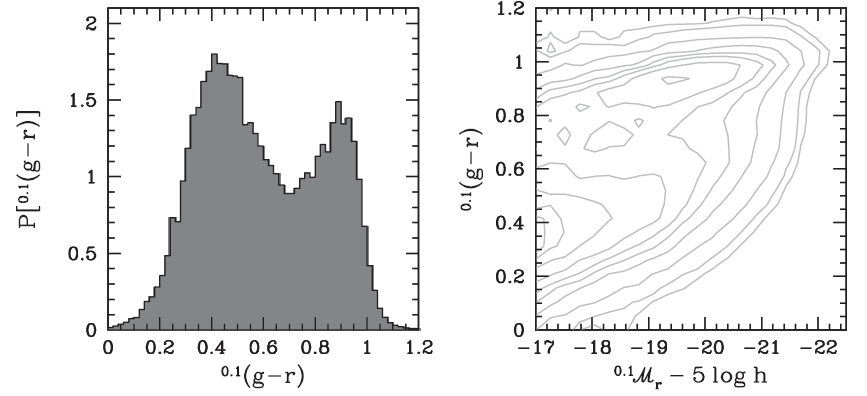
\includegraphics[width=0.9\textwidth]{images/color_bimodality.png}
    \caption{To the left: The probability density of colors of over 350 000 galaxies in the Sloan Digital Sky Survey. To the right: The color-magnitude relation for the same galaxies, clearly showing two distinct populations. Credit: \cite{Mo2010}}.
    \label{color_bimodality}
\end{figure}

\subsubsection{Supermassive Black Holes}
Almost every large galaxy with a spheroidal component has a supermassive black hole (SMBH) in its center. These are black holes with masses over $10^6 M_{\odot}$ and even above $10^9 M_{\odot}$. The mass of the SMBH correlates surprisingly well with other properties of the galaxy, such as the velocity dispersion and luminosity. This is surprising because the SMBH only has a gravitational influence within a very small radius compared to the entire galaxy, which suggests that the SMBH evolves along with the galaxy and that their formation is linked. In fact, it seems very likely that these gigantic black holes play a vital role in galaxy evolution, and are a central component of the galaxy as a whole.